\documentclass[a4paper]{article}
\usepackage{import}
\usepackage[utf8]{inputenc}
\usepackage[T1]{fontenc}
\usepackage{textcomp}
\usepackage[italian]{babel}
\usepackage{amsmath, amssymb}
\usepackage{booktabs,xltabular}
\usepackage{amsfonts}
\usepackage{subcaption}
\usepackage{amsthm}
\usepackage{cancel}
\usepackage{mdframed}
\usepackage{makecell}
\usepackage{float}
\usepackage{xcolor}
\usepackage{listings}
\usepackage{gensymb}
\usepackage{graphicx}
\usepackage{bodeplot}
\usepackage{physics}
\usepackage{tikz}
\usetikzlibrary{shapes, arrows, automata, petri, decorations.markings, decorations.pathreplacing, positioning, calc, quotes}
\usepackage{circuitikz}
\usepackage[label=corner]{karnaugh-map}
\graphicspath{{./figures/}}

% Set default font to sans-serif
\renewcommand{\familydefault}{\sfdefault} 
\usepackage{eulervm}

\usepackage{forest}

\usepackage{mathtools}
\DeclarePairedDelimiter\ceil{\lceil}{\rceil}
\DeclarePairedDelimiter\floor{\lfloor}{\rfloor}

% \usepackage{ntheorem}

\usepackage{import}
\usepackage{pdfpages}
\usepackage{transparent}
\usepackage{xcolor}

\usepackage{hyperref}
\hypersetup{
    colorlinks=false,
}

% Code blocks
\definecolor{codegreen}{rgb}{0,0.6,0}
\definecolor{codegray}{rgb}{0.5,0.5,0.5}
\definecolor{codepurple}{rgb}{0.58,0,0.82}
\definecolor{backcolour}{rgb}{0.95,0.95,0.95}

\lstdefinestyle{mystyle}{
	backgroundcolor=\color{backcolour},
	commentstyle=\color{codegreen},
	keywordstyle=\color{magenta},
	numberstyle=\tiny\color{codegray},
	stringstyle=\color{codepurple},
	basicstyle=\ttfamily\footnotesize,
	breakatwhitespace=false,
	breaklines=true,
	captionpos=b,
	keepspaces=true,
	numbers=left,
	numbersep=5pt,
	showspaces=false,
	showstringspaces=false,
	showtabs=false,
	tabsize=2
}

\lstset{style=mystyle}

\usepackage{color}
\usepackage{import}
\usepackage{pdfpages}
\usepackage{transparent}
\usepackage{xcolor}

% Example frame
\theoremstyle{definition}
\newmdtheoremenv[%
	linecolor=gray,leftmargin=0,%
	rightmargin=0,
	innertopmargin=8pt,%
	innerbottommargin=8pt,
	ntheorem]{example}{Esempio}[section]

% Important definition frame
\theoremstyle{definition}
\newmdtheoremenv[%
	linecolor=gray,leftmargin=0,%
	rightmargin=0,
	backgroundcolor=gray!40,%
	innertopmargin=8pt,%
	innerbottommargin=8pt,
	ntheorem]{definition}{Definizione}[section]

% Exercise frame
\theoremstyle{definition}
\newmdtheoremenv[%
	linecolor=gray,leftmargin=0,%
	rightmargin=0,
	innertopmargin=8pt,%
	innerbottommargin=8pt,
	ntheorem]{exercise}{Esercizio}[section]

% Theorem frame
\theoremstyle{definition}
\newmdtheoremenv[%
  linecolor=gray,leftmargin=0,%
  rightmargin=0,
  innertopmargin=8pt,%
  innerbottommargin=8pt,
  ntheorem]{theorem}{Teorema}[section]

\theoremstyle{definition}
\newmdtheoremenv[%
  linecolor=white,leftmargin=0,%
  rightmargin=0,
  innertopmargin=8pt,%
  innerbottommargin=8pt,
  ntheorem]{define}{Definizione utile}[section]

% figure support
\usepackage{import}
\usepackage{xifthen}
\pdfminorversion=7
\usepackage{pdfpages}
\usepackage{transparent}
\newcommand{\incfig}[1]{%
	\def\svgwidth{\columnwidth}
	\import{./figures/}{#1.pdf_tex}
}

% FSM tikz
\tikzset{
    place/.style={
        circle,
        thick,
        draw=black,
        minimum size=6mm,
    },
        state/.style={
        circle,
        thick,
        draw=black,
        fill=white,
        minimum size=6mm,
    },
}

\pdfsuppresswarningpagegroup=1

\usepackage{pgfplots}
\pgfplotsset{compat=1.18,width=10cm}

% Save plots as pdf and reuse them without compiling every time
\usetikzlibrary{external}
\tikzexternalize[prefix=figures/tikz/, optimize=false]


\begin{document}

\begin{titlepage}
	\begin{center}
		\vspace*{1cm}

		\Huge
		\textbf{Probabilità e Statistica\\Esercizi}

		\vspace{0.5cm}
		\LARGE
		UniVR - Dipartimento di Informatica

		\vspace{1.5cm}

		\textbf{Fabio Irimie}

		\vfill


		\vspace{0.8cm}


		2° Semestre 2023/2024

	\end{center}
\end{titlepage}


\tableofcontents
\pagebreak

\section{Introduzione}
\subsection{Cos'è l'informatica?}
È una scienza che studia la calcolabilità, cioè cerca di capire che problemi si possono
risolvere con un programma. Nasce dall'unione di matematica, ingegneria e logica. Il
computer è solo uno strumento, mentre la matematica è il linguaggio con cui si
creano algoritmi che permettono di risolvere i problemi.

\subsection{Origini dell'informatica}
Hilbert, nel 1900, si pose l'obiettivo di formalizzare tutta la matematica con un insieme
finito e non contraddittorio di assiomi. Nel 1931, invece, Gödel dimostrò che l'informatica
non potrà mai rappresentare tutta la matematica, perché ci saranno sempre proposizioni
vere ma non dimostrabili tramite il calcolo. Ci si iniziò a chiedere se esistessero
modelli di calcolo meccanici in grado di risolvere tutti i problemi. Nel 1936, Turing
propose la macchina di Turing, una \textbf{sola} macchina programmabile in grado di
risolvere tutti i problemi risolvibili:
\[
  Int(P,x) = \begin{cases}
    P(x) & \text{se } P(x) \text{ termina}\\
    \uparrow & \text{se } P(x) \text{ non termina}
  \end{cases}
\] 
dove $P$ è un programma e $x$ è un input. La macchina di Turing è un modello teorico
di calcolatore, che non esiste fisicamente, ma è in grado di simulare qualsiasi altro
calcolatore. Da questo modello deriva la concezione di calcolabilità, cioè se un problema
è intuitivamente calcolabile, allora esiste un programma in grado di risolverlo.

Altri modelli di calcolo che sono stati proposti sono:
\begin{itemize}
  \item Lambda-calcolo
  \item Funzioni ricorsive
  \item Linguaggi di programmazione (Turing-completi)
\end{itemize}

\begin{define}
  La Turing-completezza è la proprietà di un linguaggio di programmazione di essere
  in grado di simulare una macchina di Turing, cioè di poter risolvere qualsiasi problema
  risolvibile.
\end{define}

\subsubsection{Calcolabilità}
Un programma è calcolabile se termina, ma non è detto che termini in un tempo ragionevole.
Non esistono algoritmi che possono dire se un programma termina o meno. Questo è un esempio
di problema non calcolabile.

I problemi non calcolabili sono infinitamente più numerosi di quelli calcolabili

\subsection{Nozioni di base}
\subsubsection{Basi di logica}

Alcune nozioni di logica che ci serviranno in seguito:

\begin{itemize}
    \item \textbf{Linguaggio del primo ordine:} 
    \begin{itemize}
        \item Simboli relazionali $(p,q, ...)$
        \item Simboli di funzione $(f,g, ...)$
        \item Simboli di costante $(c,d, ...)$
    \end{itemize}
    \item \textbf{Simboli logici:}
    \begin{itemize}
        \item Parentesi (,) e virgola
        \item Insieme numerabile di variabili $(v,x,...)$
        \item Connettivi logici ($\neg, \land, \lor, \rightarrow, \leftrightarrow$)
        \item Quantificatori ($\forall, \exists$)
    \end{itemize}
    \item \textbf{Termini:}
        \begin{itemize}
            \item Variabili
            \item Costanti
            \item $f$ simbolo di funzione m-ario $t_1, t_2, \dots, t_m$ termini, allora

              $f(t_1, t_2, \dots, t_m)$ è un termine.
        \end{itemize}
    \item \textbf{Formula atomica:} $p$ simbolo di relazione n-ario, 
    $t_1,t_2,\dots,t_n$ 
    termini, allora $p(t_1,t_2,\dots,t_n)$ è una formula atomica.
    \item \textbf{Formula:}
    \begin{itemize}
        \item Formula atomica
        \item $\phi$ formula, allora $\neg \phi$ è una formula
        \item $\phi$ e $\psi$ formule, allora $(\phi \land \psi)$, $(\phi \lor \psi)$, $(\phi \rightarrow \psi)$, $(\phi \leftrightarrow \psi)$ sono formule.
        \item $\phi$ formula e $v$ variabile, alloar e $\forall v . \phi$ e $\exists v . \phi$ sono formule.
    \end{itemize}
\end{itemize}

\subsubsection{Nozioni sugli insiemi}

\begin{itemize}
    \item $x \in A$ signfiica che $x$ è un elemento dell'insieme $A$
    \item $\{x | P(x)\}$ si identifica insieme costuito dagli $x$ che soddisfano la proprietà (o predicato) $P(x)$
    \item $A \subseteq B$ significa che $A$ è un sottoinsieme di $B$ se ogni elemento di $A$ è anche in $B$
    \item $\mathcal{P}(S)$ denota l'insieme delle parti di $S$, ovvero l'insieme di tutti i sottoinsiemi di $S$ ($\mathcal{P}(S) = \{X | X \subseteq S\}$)
    \item $A \backslash B = \{x | x \in A \land x \notin B\}, A \cup B = \{x | x \in A \lor x \in B\}, A \cap B = \{x | x \in A \land x \in B\}$   
    \item $|A|$ denota la cardinalità di $A$, ovvero il numero di elementi in $A$.
    \item $\bar{A}$ denota il complemento di $A$, ovvero $x \bar{\in} A \leftrightarrow x \notin A$
\end{itemize}

\subsubsection{Nozioni sulle relazioni}

\begin{itemize}
    \item Prodotto cartesiano:
      \[
        A_1 \times A_2 \times \dots \times A_n = \{\langle a_1,a_2,\dots,a_n \rangle | a_1 \in A_1,\dots, a_n \in A_n\}
      \]
    \item Una \textbf{relazione} (binaria) è un sottoinsieme del prodotto cartesiano di (due) insiemi; dati $A$ e $B$, $R \subseteq A \times B$ 
    è una relazione su $A$ e $B$ 
    \begin{itemize}
        \item \textbf{Riflessiva:} $\forall a \in S$ si ha che $aRa$
        \item \textbf{Simmetrica:} $\forall a,b \in S$ se $aRb$ allora $bRa$
        \item \textbf{Antisimmetrica:} $\forall a,b \in S$ se $aRb$ e $bRa$ allora $a=b$
        \item \textbf{Transitiva:} $\forall a,b,c \in S$ se $aRb$ e $bRc$ allora $aRc$
    \end{itemize}  
    \item Per ogni relazione $R \subseteq S \times S$ la chiusura transitiva di $R$ è il più piccolo 
    insieme $R^*$ tale che $\langle a,b \rangle \in R \land \langle b,c \rangle \in R \rightarrow \langle a,c \rangle \in R^*$  
    \item Una relazione è detta \textbf{totale} su $S$ se $\forall a,b \in S$ si ha che $aRb \lor bRa$
    \item Una relazione $R$ di \textit{di equivalenza} è una relazione binaria riflessiva, simmetrica e transitiva.
    \item Una relazione binaria $R \subseteq S \times S$ è un \textbf{pre-ordine} se è riflessiva e transitiva.
    \item $R$ è un ordine parziale se è un pre-ordine antisimmetrico.
    \item $x \in S$ è \textbf{minimale} rispetto a $R$ se $\forall y \in S . y \not{R} x$ (ovvero $\neg(yRx))$
    \item $x \in S$ è \textbf{minimo} rispetto a $R$ se $\forall y \in S . xRy$
    \item $x \in S$ è \textbf{massimale} rispetto a $R$ se $\forall y \in S . x \not{R} y$ (ovvero $\neg(xRy)$)
    \item $x \in S$ è \textbf{massimo} rispetto a $R$ se $\forall y \in S . yRx$
\end{itemize}

\subsubsection{Nozioni sulle funzioni}

\begin{itemize}
    \item Una relazione $f$ è una \textbf{funzione} se $\forall a \in A$ esiste uno ed un solo $b \in B$ tale che $(a,b) \in f$
    \item $A$ dominio e $B$ codominio di $f$. Il range di $f$ è l'insieme di tutti i valori che $f$ può assumere.
    \item f è \textbf{iniettiva} se $\forall a_1,a_2 \in A$ se $a_1 \neq a_2$ allora $f(a_1) \neq f(a_2)$
    \item Se $f : A \mapsto B$ è sia iniettiva che suriettiva allora è \textbf{biiettiva} e quindi esiste $f^{-1} : B \mapsto A$ 
\end{itemize}

\section{Funzioni calcolabili}
Un insieme è una proprietà ed è rappresentato da una funzione che indica se un elemento
appartiene o meno all'insieme. I problemi da risolvere (in questo corso) hanno come
soluzione una funzione sui naturali:
\[
  f : \mathbb{N} \to \mathbb{N}
\] 
Questo tupo di funzione è un \textbf{insieme} di associazioni input-output. Un esempio
è la funzione quadrato:
\[
  f = \text{quadrato} = \{(0,0), (1,1), (2,4), (3,9), \ldots\} = \{(n,n^2) | n \in \mathbb{N}\}
\] 
Quindi \( f \) è un insieme di coppie in \( \mathbb{N} \subseteq \mathbb{N} \times \mathbb{N} \) la
cui cardinalità è: \( \left| \mathbb{N} \times \mathbb{N} \right| =
\left| \mathbb{N} \right| \). Di conseguenza la funzione è un sottoinsieme di \( \mathbb{N}
\times \mathbb{N}\):
\[
  f \subseteq \mathbb{N} \times \mathbb{N} \quad f \in \mathcal{P}(\mathbb{N} \times \mathbb{N})
\] 
Dove \( \mathcal{P}(\mathbb{N} \times \mathbb{N}) \) è l'insieme delle parti di \( \mathbb{N}
\times \mathbb{N} \), cioè l'insieme di tutti i sottoinsiemi di \( \mathbb{N} \times
\mathbb{N} \).

Il numero di funzioni è:
\[
  f: \mathbb{N} \to \mathbb{N} = \left| \mathcal{P}(\mathbb{N} \times \mathbb{N}) \right| 
  = \left| \mathcal{P}(\mathbb{N}) \right| 
\] 
\begin{example}
  Un esempio di insieme delle parti per l'insieme \( A = \{1,2,3\} \) è:
  \[
    \mathcal{P}(A) = \{\emptyset, \{1\}, \{2\}, \{3\}, \{1,2\}, \{1,3\}, \{2,3\}, \{1,2,3\}\}
  \] 
  E le cardinalità sono:
  \[
    \left| A \right| = 3 \quad \left| \mathcal{P}(A) \right| = 8 = 2^3
  \] 
  \[
    \downarrow
  \] 
  \[
    \left| \mathbb{N} \right| = \omega < 
    \underbrace{\left| \mathcal{P}(\mathbb{N}) \right| = 2^{\omega}}_{%
      \substack{\text{Insieme delle funzioni,}\\ 
      \text{non numerabile}}
    }
    = \left| \mathbb{R} \right| 
  \] 
\end{example}
Si ha quindi che \textbf{l'insieme delle funzioni non è numerabile}

\vspace{1em}
\noindent
Ci si chiede se queste funzioni sono tutte calcolabili:
\begin{definition}
  Una funzione \textbf{intuitivamente calcolabile} è una funzione descrivibile attraverso
  un algoritmo, cioè una sequenza finita di passi discreti elementari.
\end{definition}

\subsection{Quante funzioni numerabili ci sono?}
Consideriamo \( \Sigma \) come un alfabeto finito, cioè una seguenza di simboli
utilizzabili per scrivere un programma o algoritmo.
\[
  \Sigma = \{s_1,s_2,s_3, \ldots, s_n\}
\] 
\[
  \downarrow
\] 
\[
  \text{Programma} \subseteq \text{sqeuenze di simboli in } \Sigma
\] 
Con \( \Sigma^* \) si descrive l'insieme di tutte le sequenze finite di simboli in \( \Sigma \),
quindi l'insieme di tutti i possibili programmi è:
\[
  \text{Programmi} \subseteq \Sigma^*
\]

\begin{example}
  Se \( \Sigma = \left\{ a, b, c \right\} \) allora la sequenza di tutti i possibili
  simboli è:
  \[
    \Sigma^* = \{\epsilon, a, b, c, aa, ab, ac, ba, bb, bc, ca, cb, cc, aaa, aab, \ldots\}
  \]
  dove \( \epsilon \) è la stringa vuota.

  La cardinalità di \( \Sigma^* \) è infinita numerabile (anche se \( \Sigma  \) è finito).
  \[
    \left| \Sigma^* \right| = \left| \mathbb{N} \right| 
  \] 
\end{example}

Si ha quindi che l'insieme dei programmi è numerabile:
\[
  \left| \text{Programmi in } \Sigma \right| \leq \left| \Sigma^* \right| = \left| \mathbb{N} \right|
\] 
e questo implica che l'insieme delle \textbf{funzioni calcolabili è numerabile}

\begin{figure}[H]
  \centering
  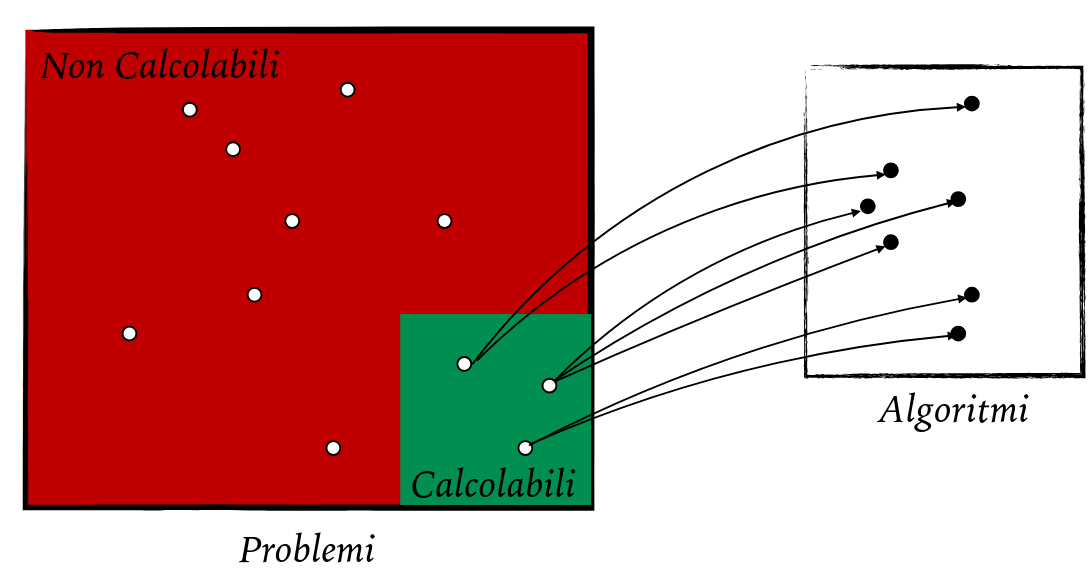
\includegraphics[width=0.8\textwidth]{cardinalita_funzioni_calcolabili}
  \caption{Cardinalità delle funzioni}
\end{figure}

\begin{example}
  Prendiamo ad esempio la seguente funzione (serie di fibonacci):
  \[
    f(n) \subseteq \mathbb{N} \times \mathbb{N}
  \] 

  \vspace{1em}
  \noindent
  Dove:
  \[
    f(0) = 1, f(1) = 1, f(2) = 2
  \] 
  \[
    f(3) = 3, f(4) = 5, f(5) = 8
  \] 
  \[
    f(6) = 13, f(7) = 21, \ldots
  \] 
  Definiamo un algoritmo ricorsivo:
  \[
    \begin{cases}
      f(0) = 1 = f(1)\\
      f(x+2) = f(x+1) + f(x)
    \end{cases}
  \] 

  \vspace{1em}
  \noindent
  Trovare un algoritmo non è possibile per tutte le funzioni, ma solo per quelle calcolabili.
\end{example}
Nell'insieme delle funzioni calcolabili ci sono:
\begin{itemize}
  \item Funzioni totali, cioè definite per ogni input \( n \in \mathbb{N} \) e terminano
    sempre
  \item Funzioni parziali, cioè non definite per ogni \( n \in \mathbb{N} \)
\end{itemize}

\subsection{Funzioni vs Insiemi}
Una funzione può essere vista come un linguaggio \( \mathcal{L}_f \) tale che:
\[
  f: \mathbb{N} \to \mathbb{N} \quad \leftrightarrow \quad
  \mathcal{L}_f = \left\{ 1^{f(x)} \;\left|\; x \in \mathbb{N} \right.\right\} \quad
  \Sigma = \{1\}
\] 
Questo linguaggio permette di dire se un input appartiene o meno al linguaggio:
\[
  \sigma  \in \Sigma^*
\] 
\[
  \downarrow
\] 
\[
  \begin{cases}
    \sigma  \in \mathcal{L}_f \quad \text{se appartiene al linguaggio}\\
    \sigma  \notin \mathcal{L}_f \quad \text{se non appartiene al linguaggio}
  \end{cases}
\] 
Parliamo di insiemi invece che di funzioni dove gli elementi dell'insieme dipendono dal
calcolo della funzione.
\begin{example}
  Prendiamo ad esempio le seguenti funzioni:
  \begin{itemize}
    \item Funzione costante (Finite)
      \[
        f(x) = 2 \to \mathcal{L}_f \text{ è finito}
      \] 
    \item Funzione lineare (Regolari)
      \[
        f(x) = 2x \to \mathcal{L}_f \text{ è infinito numerabile}
      \]
      C'è bisogno di una memoria finita per determinare se la stringa appartiene al linguaggio
    \item (Context free)
      \[
        f(\sigma) = \sigma \sigma^{\text{reverse}}
      \] 
      \[
        \sigma = abc \quad \sigma^\text{reverse} = cba
      \] 
      Per calcolare questa funzione c'è bisogno di una memoria illimitata, cioè non
      si può sapere a priori quanta ce n'è bisogno, è sufficiente uno stack.

    \item Decidibile
      \[
        f(x) = x^2
      \] 
      Per calcolare questa funzione c'è bisogno di una memoria illimitata
  \end{itemize}
\end{example}

\vspace{1em}
\noindent
Le funzioni calcolabili sono divise in classi secondo la gerarchia di Chomsky:
\begin{figure}[H]
  \centering
  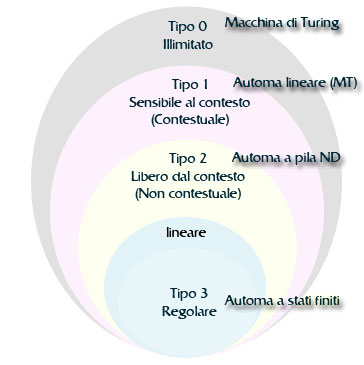
\includegraphics[width=0.7\textwidth]{gerarchia_chomsky}
  \caption{Gerarchia di Chomsky}
\end{figure}

\section{Principio di induzione}
Il principio di induzione è un meccanismo di definizione e dimostrazione che funziona
\textbf{solo su insiemi infiniti}. Esistono due metodi di induzione:
\begin{itemize}
  \item Induzione matematica
  \item Induzione strutturale
\end{itemize}
In questo corso tratteremo solo l'induzione matematica.

\vspace{1em}
\noindent
Un insieme \( A \) infinito con una relazione di ordine non riflessiva (senza l'uguale
perchè l'elemento non è in relazione con sè stesso): \( < \;: (A, <) \).
\( A = \mathbb{N} \) e \( < \) è l'ordinamento
stretto tra numeri naturali. La relazione di ordine deve essere \textbf{ben fondata},
quindi non devono esserci catene discendenti infinite, cioè una sequenza di elementi in
ordine decrescente infinita:
\[
  a_0 > a_1 > a_2 > a_3 > \ldots \to \text{non ben fondata}
\] 
Una relazione di ordine riflessiva non è ben fondata, perchè esistono catene
infinite:
\[
  a_0 \geq a_1 \geq a_2 \geq a_3 \geq a_3 \geq a_3 \geq \ldots \to \text{non ben fondata}
\]

\( b \) minimale in \( A : b \in A \) \( b \) è minimale se \( \forall b' < b \;.\; b' \notin A \) 
Ad esempio: \( \left\{ 1, 2, 3 \right\} \) ha come minimali (di contenimento) \( \left\{ 1, 2 \right\} \) 
e \( \left\{ 2,3 \right\} \).

\begin{definition}[Principio di induzione]
  Se \( A \) è un insisme ben fondato (con ordinamento \( < \)), e \( \Pi  \) è una
  proprietà definita sugli elementi di \( A: \Pi \subseteq A \), allora:
  \[
    \forall  a \in A \;.\; \underbrace{\Pi(a) }_{a\text{ soddisfa } \Pi} \iff
    \underbrace{
      \forall a \in A \;.\; \left[ \left[ \forall b < a \;.\; \Pi(b) \right] \Rightarrow
      \Pi(a)\right]
    }_{
      \substack{
        \text{Se dimostriamo } \Pi \text{ per ogni }\\
        \text{elemento più piccolo di } a, \\
        \text{allora } \Pi \text{ vale anche per } a
      }
    }
  \] 
  Consideriamo come caso base gli elementi minimali di \( A \):
  \[
    \text{Base}_A = \left\{ a \in A \;\left|\; a \text{ minimale}  \right.\right\}
  \] 
  Se si dimostra che \( \Pi \) vale per tutti gli elementi minimali di \( A \) (la base):
  \[
    \overbrace{
      \underbrace{
        \forall a \in \text{Base}_A \;.\; \Pi(a)
      }_{
        \substack{
          \text{Dimostriamo } \Pi \text{ per ogni }\\
          \text{elemento minimale di } A
        }
      }
    }^{\text{Base}}
    \wedge 
    \underbrace{
      \forall a \in A \setminus \text{Base}_A
    }_{
      \text{Passo induttivo}
    }
    \;.\;
    \underbrace{
      \forall b < a \;.\; \Pi(b)
    }_{
      \text{Ipotesi induttiva}
    }
    \underbrace{
      \Rightarrow \Pi(a)
    }_{
      \text{Tesi da dimostrare}
    }
  \] 
\end{definition}
\begin{example}
  Dimostriamo che:
  \[
    \forall n \in \mathbb{N} \sum_{i=1}^{n} i = \frac{n(n+1)}{2}
  \] 
  L'insieme è:
  \[
    A = \mathbb{N} \setminus \{0\} = \{1,2,3, \ldots\}
  \] 
  \begin{itemize}
    \item \textbf{Base}
      \[
        \text{Base}_A = \{1\}
      \] 
      \begin{itemize}
        \item dimostriamo la base
          \[
            \sum_{i=1}^{1} i = n(n+1)/2 = 1(1+1)/2 = 1
          \] 
      \end{itemize}

    \item \textbf{Passo induttivo}:
      \vspace{1em}
      \noindent
      Prendo \( n \in \mathbb{N} \) 
      \begin{itemize}
        \item Ipotesi induttiva, cioè per ogni \( m < n \) vale la proprietà:
          \[
            \forall \underset{\in \mathbb{N}}{m} < n \;.\; \sum_{i=1}^{m} i =
            \frac{m(m+1)}{2}
          \] 
          Dobbiamo dimostrare la proprietà per \( n \):
          \[
            \sum_{i=1}^{n} i = \sum_{i=1}^{n-1} i + n
          \] 
          \[
            n - 1 < n \quad \text{quindi vale l'ipotesi induttiva}
          \] 
          \[
            \sum_{i=1}^{n-1} i = \frac{(n-1)(n-1+1)}{2} = \frac{(n-1)n}{2}
          \] 
          \[
            \downarrow
          \] 
          \[
            \begin{aligned}
              \sum_{i=1}^{n} i &= \sum_{i=1}^{n-1} i + n\\
                               &= \frac{(n-1)n}{2} + n\\
                               &= \frac{(n-1)n + 2n}{2}\\
                               &= \frac{n^2 - n + 2n}{2}\\
                               &= \frac{n(n+1)}{2} \quad \square
            \end{aligned}
          \] 
      \end{itemize}
  \end{itemize}
  È quindi dimostrato che:
  \[
    \forall n \in \mathbb{N} \sum_{i=1}^{n} i = \frac{n(n+1)}{2}
  \]
\end{example}

\subsection{Linguaggi formali}
\begin{definition}
  Un linguaggio formale è un insieme di stringhe costruite su un alfabeto finito \( \Sigma  \) .
\end{definition}
Solitamente un linguaggio formale \( \mathcal{L} \) è un sottoinsieme di \( \Sigma^* \),
tipicamente infiniti, ma non necessariamente:
\[
  \mathcal{L} \subseteq \Sigma^*
\] 
I linguaggi sono divisi in:
\begin{itemize}
  \item Linguaggi finiti
  \item Linguaggi regolari, il modello utilizzato è l'automa a stati finiti.
\end{itemize}
\begin{figure}[H]
  \centering
  \begin{tikzpicture}
    \draw[thick] (0,0) circle(3);
    \draw[thick] (0,1.9) circle(1);
    \node at (4,1.9) {Linguaggi formali};
    \draw[<-, thick] (0,1.9) -- (2.6,1.9);

    \node at (5,0) {Linguaggi regolari};
    \draw[<-, thick] (0,0) -- (3.6,0);
  \end{tikzpicture}
  \caption{Linguaggi formali e linguaggi regolari}
\end{figure}

\subsection{Linguaggi regolari (automi a stati finiti, DFA)}
Il meccanismo più semplice per una memoria finita è l'automa a stati finiti

\vspace{1em}
\noindent
Consideriamo il linguaggio:
\[
\mathcal{L}_f = \left\{ 1^{2n} \;\left|\; n \in \mathbb{N} \right. \right\}
\] 
ha bisogno di due stati \( q_0 \) e \( q_1 \). Lo stato \( q_0 \) rappresenta
l'informazione di essere di lunghezza pari, mentre lo stato \( q_1 \)
rappresenta l'informazione di essere di lunghezza dispari.
\begin{figure}[H]
  \centering
  \begin{tikzpicture}[node distance=3cm, on grid, auto]
    \node[state, initial, accepting] (q0) {$q_0$};
    \node[state, right of=q0] (q1) {$q_1$};

    \draw (q0) edge[bend left, above] node{1} (q1);
    \draw (q1) edge[bend left, below] node{1} (q0);
  \end{tikzpicture}
  \caption{Automa a stati finiti per il linguaggio \( \mathcal{L}_f = \left\{ 1^{2n} \;\left|\; n
            \in \mathbb{N} \right. \right\} \)}
\end{figure}
L'automa a stati finiti \textbf{deterministico} è definito come una quintupla: 
\[
  M = \left( Q, \Sigma , \delta, q_0, F \right) 
\] 
dove:
\begin{itemize}
  \item \( Q \) è un insieme \textbf{finito} di stati. Ogni stato rappresenta
    un'informazione

  \item \( \Sigma  \) è un insieme \textbf{finito} di simboli (alfabeto).
    Ogni simbolo è un elemento atomico che posso leggere e che compone le
    stringhe da riconoscere
    
  \item \( q_0 \in Q \) è uno stato e identifica lo stato iniziale. Lo stato finale
    viene indicato con un doppio cerchio

  \item \( F \subseteq Q \) è l'insieme degli stati finali (di accettazione)

  \item \( \delta: Q \times \Sigma \to Q \) È una \textbf{funzione di transizione}
    che dato uno stato e un simbolo, restituisce lo stato successivo ed è come se
    fosse una tabella che associa ad ogni coppia (stato, simbolo) uno stato:
    \begin{table}[H]
      \centering
      \begin{tabular}{c|c|c}
        \( \Sigma \setminus Q\) & \( q_0 \) & \( q_1 \)\\
        \hline
        1 & \( q_1 \) & \( q_0 \)\\
      \end{tabular}
    \end{table}
    La funzione deve essere \textbf{totale}, cioè deve essere definita per ogni
    coppia \( (q,a) \in Q \times \Sigma  \), quindi la tabella deve essere completa.

  \item \( \hat{\delta}: Q \times \Sigma^* \to Q \) Descrive lo stato che raggiungono
    leggendo una sequenza di simboli
    \[
      \begin{cases}
        \hat{\delta}(q, \epsilon) = q\\
        \hat{\delta}(q, wa) = \delta(\hat{\delta}(q,w), a)
      \end{cases}
      \quad
      w \in \Sigma^*, \quad a \in \Sigma 
    \] 
    È quindi la \textbf{chiusura transitiva} di \( \delta \)
\end{itemize}

\subsubsection{Come si dimostra che un linguaggio è regolare?}
\begin{example}
  Prendiamo in considerazione il seguente linguaggio:
  \[
    L = \left\{ \sigma  \;\left|\; \sigma \text{ contiene almeno due } 1 \right. \right\}
  \] 
  \[
    \Sigma = \{0,1\}
  \] 
  Con le seguenti stringhe si ha:
  \begin{itemize}
    \item \( \sigma = 011 \in \mathcal{L} \) 
    \item \( \sigma = 1000100 \in \mathcal{L} \) 
    \item \( \sigma = 00010 \notin \mathcal{L} \) 
  \end{itemize}
  L'informazione che codifica lo stato iniziale deve essere coerente con \( \varepsilon  \) 
  (stringa vuota)
  \begin{figure}[H]
    \centering
    \begin{tikzpicture}[->, node distance=2cm, on grid, auto]
      \node[state, initial] (q0) {$q_0$};
      \node[state, right of=q0] (q1) {$q_1$};
      \node[state, right of=q1, accepting] (q2) {$q_2$};

      \draw (q0) edge[above] node{1} (q1);
      \draw (q0) edge[loop above] node{0} (q0);
      \draw (q1) edge[loop above] node{0} (q2);
      \draw (q1) edge[above] node{1} (q2);
      \draw (q2) edge[loop above] node{0,1} (q2);
    \end{tikzpicture}
    \caption{Automa a stati finiti per il linguaggio \( \mathcal{L} \)}
  \end{figure}
\end{example}
Un lingauggio \( L \) è riconosciuto da \( M = \left( Q, \Sigma, \delta, q_0, f \right)  \) (DFA, Deterministic Finite Automaton) se:
\( L = L(M) \) dove \( L(M) \) è il linguaggio di \( M \) definito come:
\[
  L(M) = \left\{ \sigma  \in \Sigma^* \;\left|\; \hat{\delta}(q_0, \sigma) \in F \right. \right\}
\] 
Cioè sono tutte le stringhe che partendo da \( q_0 \) fanno raggiungere uno stato finale.

\vspace{1em}
\noindent
\begin{definition}
  Per dimostrare che \( L \) è regolare dobbiamo costruire \( M \) (almeno un \( M \)) e
  \textbf{dimostrare che} \( L = L(M) \) 
\end{definition}
\( L = L(M) \) è un uguaglianza insiemistica e si dimostra con due contenimenti:
\[
  L = L(M) \equiv L \subset L(M) \wedge L(M) \subset L
\]  
\begin{itemize}
  \item Se un elemento si trova nel primo insieme, allora si trova anche nel secondo
    \[
      L \subseteq L(M) \equiv \sigma \in L \Rightarrow \sigma \in L(M) \equiv
      \sigma \in L \Rightarrow \hat{\delta}(q_0, \sigma) \in F
    \] 
  \item Se un elemento si trova nel secondo insieme, allora si trova anche nel primo
    \[
      L(M) \subseteq L \equiv \sigma \in L(M) \Rightarrow \sigma \in L \equiv
      \hat{\delta}(q_0, \sigma) \in F \Rightarrow \sigma \in L
    \]
    o per contrapposizione:
    \[
      \sigma \notin L \Rightarrow \hat{\delta}(q_0, \sigma) \notin F
    \] 
\end{itemize}
Questo dimostra che il linguaggio è regolare perchè è riconosciuto da un automa.

\begin{example}
  Riprendendo l'esempio precedente:
  \[
    L = \left\{ \sigma \in \Sigma^* \;\left|\; \sigma \text{ contiene almeno due } 1 \right. \right\}
  \] 
  \[
    \Sigma = \{0,1\}
  \]
  \( M = \) 
  \begin{figure}[H]
    \centering
    \begin{tikzpicture}[->, node distance=2cm, on grid, auto]
      \node[state, initial] (q0) {$q_0$};
      \node[state, right of=q0] (q1) {$q_1$};
      \node[state, right of=q1, accepting] (q2) {$q_2$};

      \draw (q0) edge[above] node{1} (q1);
      \draw (q0) edge[loop above] node{0} (q0);
      \draw (q1) edge[loop above] node{0} (q2);
      \draw (q1) edge[above] node{1} (q2);
      \draw (q2) edge[loop above] node{0,1} (q2);
    \end{tikzpicture}
    \caption{Automa a stati finiti per il linguaggio \( \mathcal{L} \)}
  \end{figure}
  \noindent
  Dimostriamo per induzione sulla lunghezza delle stringhe \( \sigma \in \Sigma^* \) 
  che se \( x \in L \) allora \( \hat{\delta}(q_0, x) \in F \) e se \( x \notin L \) allora
  \( \hat{\delta}(q_0, x) \notin F \).

  \vspace{1em}
  \noindent
  \( \left| \sigma  \right| = 0 \) non è \textbf{mai} sufficiente come base, ma
  è eventualmente la base \textbf{solo} per una delle due dimostrazioni. Bisogna
  quindi prendere la lunghezza più piccola che permette di avere sia \( \sigma \in L \) 
  che  \( \sigma \notin L \), in questo caso è \( \left| \sigma  \right| = 2 \).
  Per ogni \( \sigma  \) tale che \( \left| \sigma  \right| < 2 \quad \sigma \notin L \)
  perchè non può contenere due 1 e non è riconosciuta da \( M \) dove il primo stato finale
  è raggiunto leggendo almeno due simboli.
  \[
    \varepsilon \in L \quad \varepsilon \notin L
  \] 
  \begin{itemize}
    \item \textbf{Base}: Controlliamo ogni stringa di lungheezza minima nel linguaggio per
      provare il caso base. In questo caso la lunghezza minima è
      \( \left| \sigma  \right| = 2 \) 
      \[
        \begin{cases}
          \sigma &= 11 \in L \; \text{ e } \; \hat{\delta}(q_0, 11) = q_2 \in F \\
          \sigma &= 10 \notin L \; \text{ e } \; \hat{\delta}(q_0, 10) = q_1 \notin F \\
          \sigma &= 01 \notin L \; \text{ e } \; \hat{\delta}(q_0, 01) = q_1 \notin F \\
          \sigma &= 00 \notin L \; \text{ e } \; \hat{\delta}(q_0, 00) = q_0 \notin F
        \end{cases}
      \] 

    \item \textbf{Passo induttivo}: Assumiamo che valga l'\textbf{ipotesi induttiva}, cioè
      la tesi con un limite fissato:
      \[
        \forall \sigma \in \Sigma^* \;.\; \left| \sigma  \right| \le n \;.\;
        \begin{cases}
          \sigma \in L &\Rightarrow \hat{\delta}(q_0, \sigma) \in F\\
          \sigma \notin L &\Rightarrow \hat{\delta}(q_0, \sigma) \notin F
        \end{cases}
      \] 
      Vogliamo dimostrare che la tesi vale per \( \left| \sigma  \right| = n + 1 \)
      (la successiva stringa che posso considerare).

      \noindent
      \textbf{Tesi}:
      \( 
        \begin{cases}
          \sigma \in L \Rightarrow \hat{\delta}(q_0,\sigma) = q_2
          \; \sigma \text{ contiene almeno due 1}\\
          \sigma \notin L \Rightarrow \hat{\delta}(q_0,\sigma) = q_0
          \; \sigma \text{ non contiene 1}\\
          \sigma \notin L \Rightarrow \hat{\delta}(q_0,\sigma) = q_1
          \; \sigma \text{ contiene esattamente un 1}
        \end{cases}
      \) 

      \vspace{1em}
      \noindent
      \textbf{Ipotesi induttiva}:
      \[
        \forall \sigma \in \Sigma^* \;.\; \left| \sigma  \right| \le n \;.\;
        \text{ allora la tesi vale su } \sigma
      \] 

      \vspace{1em}
      \noindent
      Dimostrazione della tesi per \( \sigma  \) tale che \( \left| \sigma  \right| = n + 1 \).
      (\( \left| \sigma' \right| = n \) quindi su \( \sigma' \) possiamo applicare l'ipotesi
      induttiva):
      \[
        \left| \sigma  \right| = n + 1 \to 
          \sigma = \sigma'1 \; \vee \; \sigma = \sigma'0
      \] 
      \begin{itemize}
        \item Supponiamo che \( \sigma  \) appartenga al linguaggio e termini con 1:
          \[
            \sigma \in L \wedge \sigma  = \sigma'1
          \] 
          \[
            \downarrow
          \] 
          \begin{itemize}
            \item Se \( \sigma' \in L \) applico l'ipotesi induttiva:
              \[
                  \hat{\delta}(q_0, \sigma') = q_2\\
              \] 
              \[
                \begin{aligned}
                  \hat{\delta}(q_0, \sigma) &\stackrel{\sigma = \sigma'1}{=}
                  \hat{\delta}(q_0, \sigma'1)\\
                                            &= \delta(\hat{\delta}(q_0, \sigma'), 1)\\
                                            &= \delta(q_2, 1) = q_2 \in F
                \end{aligned}
              \] 

            \item Se \( \sigma' \notin L \) allora \( \sigma' \) contiene esattamente un 1:
              \[
                \hat{\delta}(q_0, \sigma') = q_1
              \] 
              \[
                \hat{\delta}(q_0, \sigma'1) = \delta(q_1, 1) = q_2
              \] 
          \end{itemize}

        \item Supponiamo che \( \sigma  \) appartenga al linguaggio e termini con 0:
          \[
            \sigma \in L \wedge \sigma = \sigma'0
          \] 
          Per definizione di \( L \) abbiamo che
          \[
            \sigma \in L \wedge \sigma = \sigma'0 \Rightarrow \sigma' \in L
          \] 
          Dimostriamo l'ipotesi induttiva:
          \[
            \hat{\delta}(q_0, \sigma') = q_2
          \] 
          allora
          \[
            \begin{aligned}
              \hat{\delta}(q_0, \sigma) &= \hat{\delta}(q_0, \sigma'0)\\
                                        &= \delta(\hat{\delta}(q_0, \sigma'), 0)\\
                                        &= \delta(q_2, 0) = q_2 \in F
            \end{aligned}
          \] 

        \item Supponiamo che \( \sigma  \) non appartenga al linguaggio e contiene
          esatatmente un 1:
          \begin{itemize}
            \item \( \sigma  = \sigma'0 \Rightarrow \sigma' \notin L \) e contiene esattamente un 1\\
              \noindent
              Ipotesi induttiva:
              \[
                \hat{\delta}(q_0, \sigma') = q_1
              \] 
              \[
                \Downarrow
              \] 
              \[
                \begin{aligned}
                  \hat{\delta}(q_0, \sigma) &= \hat{\delta}(q_0, \sigma'0)\\
                                            &= \delta(\hat{\delta}(q_0, \sigma'), 0)\\
                                            &= \delta(q_1, 0) = q_1 \notin F
                \end{aligned}
              \] 

            \item \( \sigma = \sigma'1 \Rightarrow \sigma' \notin L \) e non contiene 1\\
              \noindent
              Ipotesi induttiva:
              \[
                \hat{\delta}(q_0, \sigma') = q_0
              \] 
              \[
                \Downarrow
              \] 
              \[
                \begin{aligned}
                  \hat{\delta}(q_0, \sigma) &= \hat{\delta}(q_0, \sigma'1)\\
                                            &= \delta(\hat{\delta}(q_0, \sigma'), 1)\\
                                            &= \delta(q_0, 1) = q_1 \notin F
                \end{aligned}
              \] 
          \end{itemize}

        \item Supponiamo che \( \sigma  \) non appartenga al linguaggio e non contiene 1
          \[
            \sigma \notin L \wedge  \sigma  = \sigma'0
          \] 
          \( \sigma = \sigma'1 \) non è possibile per l'ipotesi che \( \sigma  \) non contiene 1\\
          \noindent
          Ipotesi induttiva:
          \[
              \hat{\delta}(q_0, \sigma') = q_0\\
          \] 
          \[
            \Downarrow
          \] 
          \[
            \begin{aligned}
              \hat{\delta}(q_0, \sigma) &= \hat{\delta}(q_0, \sigma'0)\\
                                        &= \delta(\hat{\delta}(q_0, \sigma'), 0)\\
                                        &= \delta(q_0, 0) = q_0 \notin F
            \end{aligned}
          \] 
      \end{itemize}
  \end{itemize}
  Tutti i casi sono dimostrati, quindi abbiamo dimostrato che:
  \[
    L = L(M) \quad \Rightarrow \quad L \text{ è regolare}
  \]
\end{example}
\begin{exercise}
  Consideriamo il seguente linguaggio:
  \[
    \begin{aligned}
      L &= \left\{ \sigma \in \Sigma^* \;\left|\; \text{ogni sequenza di } 0 \text{ è di lunghezza pari} \right.\right\}\\
    \end{aligned}
  \] 
  \[
    \Sigma = \{0,1\}
  \] 
  Si può accettare anche sequenze di lunghezza 0. Alcuni esempi sono:
  \[
    \begin{aligned}
      101 \notin L\\
      1111 \in L\\
      10010000 \in L\\
      00101 \notin L\\
    \end{aligned}
  \] 
  L'automa a stati finiti \( M \) è il seguente:
  \begin{itemize}
    \item \( q_0 \): Non sono stati letti 0
    \item \( q_1 \): Sequenza di 0 consecutiva di lunghezza dispari
    \item \( q_2 \): Sequenza di 0 consecutiva di lunghezza pari
  \end{itemize}
  \begin{figure}[H]
    \centering
    \begin{tikzpicture}[->, node distance=2cm, on grid, auto]
      \node[state, initial, accepting] (q0) {$q_0$};

      \node[state, right of=q0] (q1) {$q_1$};

      \node[state, right of=q1, accepting] (q2) {$q_2$};

      \node[state, above of=q1] (q3) {$q_{\bot}$};

      \draw (q0) edge[loop above] node{1} (q0);
      \draw (q0) edge[above] node{0} (q1);
      \draw (q1) edge[bend left, above] node{0} (q2);
      \draw (q2) edge[bend left, above] node{0} (q1);
      \draw (q2) edge[loop above] node{1} (q2);
      \draw (q1) edge[left] node{1} (q3);
      \draw (q3) edge[loop above] node{0,1} (q3);
    \end{tikzpicture}
    \caption{Automa a stati finiti per il linguaggio \( L \)}
  \end{figure}
  \noindent
  La tesi è:
  \begin{itemize}
    \item \( \sigma \in L \) e non contiene 0:
      \(
        \Rightarrow \hat{\delta}(q_0, \sigma) = q_0
      \) 

    \item \( \sigma \in L \) e contiene una sequenza pari di 0:
      \(
        \Rightarrow \hat{\delta}(q_0, \sigma) = q_2
      \)

    \item \( \sigma \notin L \) e contiene una sequenza \textbf{finale} dispari di 0:
      \(
        \Rightarrow \hat{\delta}(q_0, \sigma) = q_1
      \)

    \item \( \sigma \notin L \) e contiene una sequenza dispari di 0 seguita da 1:
      \(
        \Rightarrow \hat{\delta}(q_0, \sigma) = q_{\bot}
      \)
  \end{itemize}
\end{exercise}
\begin{exercise}
  Consideriamo il seguente linguaggio (ogni sequenza di 0 è di lunghezza almeno 2):
  \[
    L = \left\{ \sigma \in \Sigma^* \;\left|\; \exists n \ge 1 \;.\; \sigma = 0^n \Rightarrow n \ge 2 \right.\right\}\\
  \] 
  \[
    \Sigma = \{0,1\}
  \]
  L'automa a stati finiti \( M \) è il seguente:
  \begin{itemize}
    \item \( q_0 \): Non contiene 0, oppure \textbf{tutte} le sequenze di 0
      sono lunghe almeno 2

    \item \( q_1 \): Esattamente uno 0
      
    \item \( q_2 \): Almeno due 0
  \end{itemize}
  \begin{figure}[H]
    \centering
    \begin{tikzpicture}[->, node distance=2cm, on grid, auto]
      \node[state, initial, accepting] (q0) {$q_0$};

      \node[state, right of=q0] (q1) {$q_1$};

      \node[state, right of=q1, accepting] (q2) {$q_2$};

      \node[state, below of=q1] (q3) {$q_{\bot}$};

      \draw (q0) edge[loop above] node{1} (q0);
      \draw (q0) edge[above] node{0} (q1);
      \draw (q1) edge[above] node{0} (q2);
      \draw (q0) edge[bend left, above] node{1} (q2);
      \draw (q2) edge[loop above] node{0} (q2);
      \draw (q1) edge[right] node{1} (q3);
      \draw (q3) edge[loop below] node{0,1} (q3);

    \end{tikzpicture}
    \caption{Automa a stati finiti per il linguaggio \( L \)}
  \end{figure}
  \noindent
  La tesi è:
  \begin{itemize}
    \item \( \sigma \in L \) e \( \sigma = \sigma'1 \)
      \(
        \Rightarrow \hat{\delta}(q_0, \sigma) = q_0
      \) 

    \item \( \sigma \in L \) e \( \sigma = \sigma'0 \) 
      \(
        \Rightarrow \hat{\delta}(q_0, \sigma) = q_2
      \) 

    \item \( \sigma \notin L \) e \( \sigma = \sigma'0 \) dove l'ultima sequenza di 0
      è esattamente lunga 1:
      \(
        \Rightarrow \hat{\delta}(q_0, \sigma) = q_1
      \) 

    \item \( \sigma \notin L \) e \( \sigma  \) contiene una sequenza lunga 1 di 0:
      \(
        \Rightarrow \hat{\delta}(q_0, \sigma) = q_{\bot}
      \)
  \end{itemize}
\end{exercise}

\subsection{Automi a stati finiti non deterministici (NFA)}
Un automa a stati finiti non deterministico si crea quando ad un solo simbolo sono
associate più transizioni. Quando questo succede gli stati vengono considerati in
parallelo. Un NFA è definito come una quintupla:
\[
  N = \left< Q, \Sigma, \delta, q_0, F \right>
\] 
\begin{itemize}
  \item \( Q \) è un insieme finito di stati
  \item \( \Sigma  \) è un insieme finito di simboli (alfabeto)
  \item \( q_0 \in Q \) è uno stato e identifica lo stato iniziale
  \item \( F \subseteq Q \) è l'insieme degli stati finali
  \item \( \delta: Q \times \Sigma \to \mathcal{P}(Q) \) è una funzione di transizione che
    dato uno stato e un simbolo restituisce un insieme di stati \textbf{potenzialmente}
    raggiungibili. È possibile che esistano coppie associate all'insieme vuoto:
    \[
      \emptyset \in \mathcal{P}(Q)
    \] 
    Inoltre non è obbligatorio avere un arco uscente per ogni simbolo di \( \Sigma \).
  \item \( \hat{\delta}: Q \times \Sigma^* \to \mathcal{P}(Q) \) Descrive gli stati che si possono
    raggiungere leggendo una sequenza di simboli:
    \[
      \begin{cases}
        \hat{\delta}(q, \epsilon) = \{q\}\\
        \hat{\delta}(q, wa) = \bigcup_{p \in \hat{\delta}(q,w)} \delta(p, a)
      \end{cases}
      \quad
      w \in \Sigma^*, \quad a \in \Sigma 
    \] 
    È quindi la chiusura transitiva di \( \delta \)
\end{itemize}
\begin{example}
  Un esempio di NFA è il seguente:
  \begin{figure}[H]
    \centering
    \begin{tikzpicture}[->, node distance=2cm, on grid, auto]
      \node[state, initial] (q0) {$q_0$};

      \node[state, above right of=q0] (q1) {$q_1$};

      \node[state, below right of=q1] (q2) {$q_2$};

      \draw (q0) edge[above] node{a} (q1);
      \draw (q0) edge[below] node{a} (q2);

    \end{tikzpicture}
    \caption{Esempio di NFA}
  \end{figure}
  \[
    \delta(q_0, a) = \{q_1, q_2\} \subseteq Q
  \] 
\end{example}

\subsubsection{Linguaggio riconosciuto da un NFA}
Un linguaggio \( L \) è riconosciuto da un NFA \( N \) se:
\[
  L(N) = \left\{ \sigma \in \Sigma^* \;\left|\;
  \hat{\delta}(q_0, a) \cap F \neq \emptyset \right.\right\}
\] 
\begin{example}
  Consideriamo il seguente linguaggio:
  \[
  L(N) = \left\{ \sigma \in \Sigma^* \;\left|\; \sigma \text{ contiene almeno due } 1 \right. \right\}
  \] 
  \begin{figure}[H]
    \centering
    \begin{tikzpicture}[->, node distance=2cm, on grid, auto]
      \node[state, initial] (q0) {$q_0$};

      \node[state, right of=q0] (q1) {$q_1$};

      \node[state, above of=q0] (q2) {$q_2$};

      \draw (q2) edge[right] node{1} (q0);
      \draw (q0) edge[bend left, below] node{1} (q1);
      \draw (q1) edge[bend left, below] node{1} (q0);

      \draw (q1) edge[below] node{1} (q2);
      \draw (q2) edge[bend left, above] node{0,1} (q1);

      \draw (q2) edge[loop above] node{0,1} (q2);

    \end{tikzpicture}
    \caption{Esempio di NFA per il linguaggio \( L \)}
  \end{figure}
\end{example}

\begin{theorem}[Teorema di Rabin-Scott]
  Ogni linguaggio riconosciuto da un NFA è riconosciuto da un DFA.
  \[
    \forall N = (Q, \Sigma, \delta, q_0, F) \; \exists M = (Q', \Sigma, \delta', q_0', F') \;.\;
    L(N) = L(M)
  \] 

  \vspace{1em}
  \noindent
  \textbf{Dimostrazione}: Consideriamo un NFA \( N = (Q, \Sigma, \delta, q_0, F) \) e
  costruiamo un DFA \( M = (Q', \Sigma, \delta', q_0', F') \).
  Gli insiemi degli stati sono:
  \[
    Q' = \mathcal{P}(Q)
  \] 
  \[
   Q = \{q_0, q_1, q_2\}
  \] 
  \[
    \Downarrow
  \] 
  \[
    Q' = \left\{ 
      \stackrel{q'_1}{\emptyset}, \stackrel{q'_0}{\{q_0\}}, \stackrel{q'_2}{\{q_1\}},
      \stackrel{q'_3}{\{q_2\}}, \stackrel{q'_4}{\{q_0, q_1\}}, \stackrel{q'_5}{\{q_0, q_2\}},
      \stackrel{q'_6}{\{q_1, q_2\}}, \stackrel{q'_7}{\{q_0, q_1, q_2\}}
    \right\}
  \] 
  Lo stato iniziale rimane uguale per entrambi gli insiemi: \( q'_0 = \{q_0\}  \).

  Gli insiemi degli stati finali sono:
  \[
    F' = \left\{ P \subseteq Q \;\left|\; P \cap F \neq \emptyset \right. \right\} \quad
    P \in \mathcal{P}(Q)
  \] 
  Quindi:
  \[
    F = \{q_2\} 
  \] 
  \[
    F' = \left\{ \stackrel{q'_3}{\{q_2\}}, \stackrel{q'_6}{\{q_1, q_2\}},
      \stackrel{q'_5}{\{q_0, q_2\}}, \stackrel{q'_7}{\{q_0, q_1, q_2\}}
    \right\}
  \] 
  La funzione di transizione è definita come:
  \[
    \delta'(P, a) = \bigcup_{q \in P} \delta(q, a) \in \mathcal{P}(Q) \quad P \in Q' = \mathcal{P}(Q),\; a \in \Sigma 
  \]
  Quindi:
  \[
    \begin{aligned}
      \underbrace{\delta'(q'_5, 1)}_{= \{q_1, q_2\} }
      &= \delta(q_1, 1) \cup \delta(q_2, 1)\\
                       &= \{q_0, q_2\} \cup \{q_0, q_1, q_2\}\\
                       &= \{q_0, q_1, q_2\} = q'_7
    \end{aligned}
  \] 

  \vspace{1em}
  \noindent
  Dimostriamo: 
  \begin{enumerate}
    \item 
      \( \hat{\delta}(q_0, \sigma) = \hat{\delta}'(q'_0, \sigma) = \{q_0\}  \) 

      \vspace{1em}
      \noindent
      Dimostriamo per induzione su \( \left| \sigma  \right|  \):

      \begin{itemize}
        \item 
          Se \( \sigma = \varepsilon \) allora:
          \[
            \hat{\delta}'(q'_0, \varepsilon) = q'_0 = \{q_0\} = \hat{\delta}(q_0, \varepsilon)
          \] 
          per le definizioni

        \item Se \( \sigma = \sigma'a \):
          \[
            \begin{aligned}
              \hat{\delta}'(q'_0, \sigma'a) &= \delta'(\hat{\delta}'(q_0, \sigma'), a)\\
                                            &= \delta'(\hat{\delta}(q_0, \sigma'), a)\\
                                            &= \bigcup_{p \in \hat{\delta}(q_0, \sigma')} \delta(p, a)\\
                                            &= \hat{\delta}(q_0, \sigma'a)
            \end{aligned}
          \] 
          Definizione di \( \hat{\delta}' \) non deterministica
      \end{itemize}
    \item
      \(
        \sigma \in L(N) \iff \sigma \in L(M)
      \) 

      \vspace{1em}
      \noindent
      Dimostriamo la definizione di linguaggio riconosciuto in NFA:
      \[
        \begin{aligned}
          \sigma \in L(N) &\iff \hat{\delta}(q_0, \sigma) \cap F \neq \emptyset\\
                          &\iff \hat{\delta}'(q'_0, \sigma) \cap F' \neq \emptyset \;(\text{(1.)})\\
                          &\iff \hat{\delta}'(q'_0, \sigma) \in F'\\
                          &\iff \sigma \in L(M) \; \text{(def. linguaggio accettato in DFA)}
        \end{aligned}
      \] 
  \end{enumerate}

\end{theorem}


\end{document}
